% THIS IS SIGPROC-SP.TEX - VERSION 3.1
% WORKS WITH V3.2SP OF ACM_PROC_ARTICLE-SP.CLS
% APRIL 2009
%
% It is an example file showing how to use the 'acm_proc_article-sp.cls' V3.2SP
% LaTeX2e document class file for Conference Proceedings submissions.
% ----------------------------------------------------------------------------------------------------------------
% This .tex file (and associated .cls V3.2SP) *DOES NOT* produce:
%       1) The Permission Statement
%       2) The Conference (location) Info information
%       3) The Copyright Line with ACM data
%       4) Page numbering
% ---------------------------------------------------------------------------------------------------------------
% It is an example which *does* use the .bib file (from which the .bbl file
% is produced).
% REMEMBER HOWEVER: After having produced the .bbl file,
% and prior to final submission,
% you need to 'insert'  your .bbl file into your source .tex file so as to provide
% ONE 'self-contained' source file.
%
% Questions regarding SIGS should be sent to
% Adrienne Griscti ---> griscti@acm.org
%
% Questions/suggestions regarding the guidelines, .tex and .cls files, etc. to
% Gerald Murray ---> murray@hq.acm.org
%
% For tracking purposes - this is V3.1SP - APRIL 2009

\documentclass{acm_proc_article-sp}

\begin{document}

\title{Text input method for single-handed mobile devices}

%
% You need the command \numberofauthors to handle the 'placement
% and alignment' of the authors beneath the title.
%
% For aesthetic reasons, we recommend 'three authors at a time'
% i.e. three 'name/affiliation blocks' be placed beneath the title.
%
% NOTE: You are NOT restricted in how many 'rows' of
% "name/affiliations" may appear. We just ask that you restrict
% the number of 'columns' to three.
%
% Because of the available 'opening page real-estate'
% we ask you to refrain from putting more than six authors
% (two rows with three columns) beneath the article title.
% More than six makes the first-page appear very cluttered indeed.
%
% Use the \alignauthor commands to handle the names
% and affiliations for an 'aesthetic maximum' of six authors.
% Add names, affiliations, addresses for
% the seventh etc. author(s) as the argument for the
% \additionalauthors command.
% These 'additional authors' will be output/set for you
% without further effort on your part as the last section in
% the body of your article BEFORE References or any Appendices.

\numberofauthors{4} %  in this sample file, there are a *total*
% of EIGHT authors. SIX appear on the 'first-page' (for formatting
% reasons) and the remaining two appear in the \additionalauthors section.
%
\author{
% You can go ahead and credit any number of authors here,
% e.g. one 'row of three' or two rows (consisting of one row of three
% and a second row of one, two or three).
%
% The command \alignauthor (no curly braces needed) should
% precede each author name, affiliation/snail-mail address and
% e-mail address. Additionally, tag each line of
% affiliation/address with \affaddr, and tag the
% e-mail address with \email.
%
% 1st. author
\alignauthor Kaith Menken\\
\email{kaith-uwe.menken@uni-ulm.de}
% 2nd. author
\alignauthor Sebastian Hartwig\\
\email{sebastian.hartwig@uni-ulm.de}
\and
% 3rd. author
\alignauthor Daniel Eischer 
\email{daniel.eischer@uni-ulm.de}
% 4th. author
\alignauthor Johann Albach\\
\email{johann.albach@uni-ulm.de}
}
\maketitle
\begin{abstract}
These days our society increasingly depends on micro computers. That is because of a wide range of functionality integrated in mobile devices. Hence, usability and performance are importand factors which are profitable to develop. Since the idea of mobile devices is communication there has been many researches in terms of text input improvement. Short message service and electronic mails aren't the only applicatios anymore using text input methods. Hot topics in terms of mobile software developement   are fault tolerance text input methods. Mobile devices that correct misspelled text for their user are highly in demand.

We proceed on the assumption that in futur the usage of mobile devices is going be more prompt than now. Meaning mobile devices will leave our pockets and integrate in our clothes or even will be placed on our body.

The idea is wearing, for instance a smartphone attached to a bracelet on our wrists. Providing instant access to the smartphone. In our approach we try to realise a text input method for single-handed mobile device usage.
\end{abstract}

\terms{Mobile Human Computer Interaction, Software Developement, Smartphone}

\keywords{smartphone, swype, single-handed, text, input, methods} % NOT required for Proceedings

\section{Introduction}
Short messages shape our daly life. Every smartphone user is writing thousands of short texts every week. Therefor software that supports users while typing is important. The tendency for futur smartphones is to be accessable more easily. Micro computers that are integrated in clothes or wearable smartphones providing instant access. Those developements require different implementation of text input methods enableing a single-handed input.

Our approach targets a device attached to the wrist of the user. Placed at the wrist of a user those devices are easilie reachable. The only challange is to compensate for a single-handed input that could in the worst case negate the promptness of our approach. Therefor we have to rethink the softkeyboard layout to shrink the hole keyboard frame occupying less of the display.

Another important feature in our approach are swype gestures. Thereby our keyboard enables advanced input options like special characters and numbers. Also no space bar as single button is planed, furthermore a single gesture should execute the space bar function. Since swype gestures are easy to perform a visceral mapping to their action is essential. Accordingly only a few frequently used functions are captured in swype gestures like changing from letters to special characters. 
\begin{figure}[htb]
  \begin{center}
    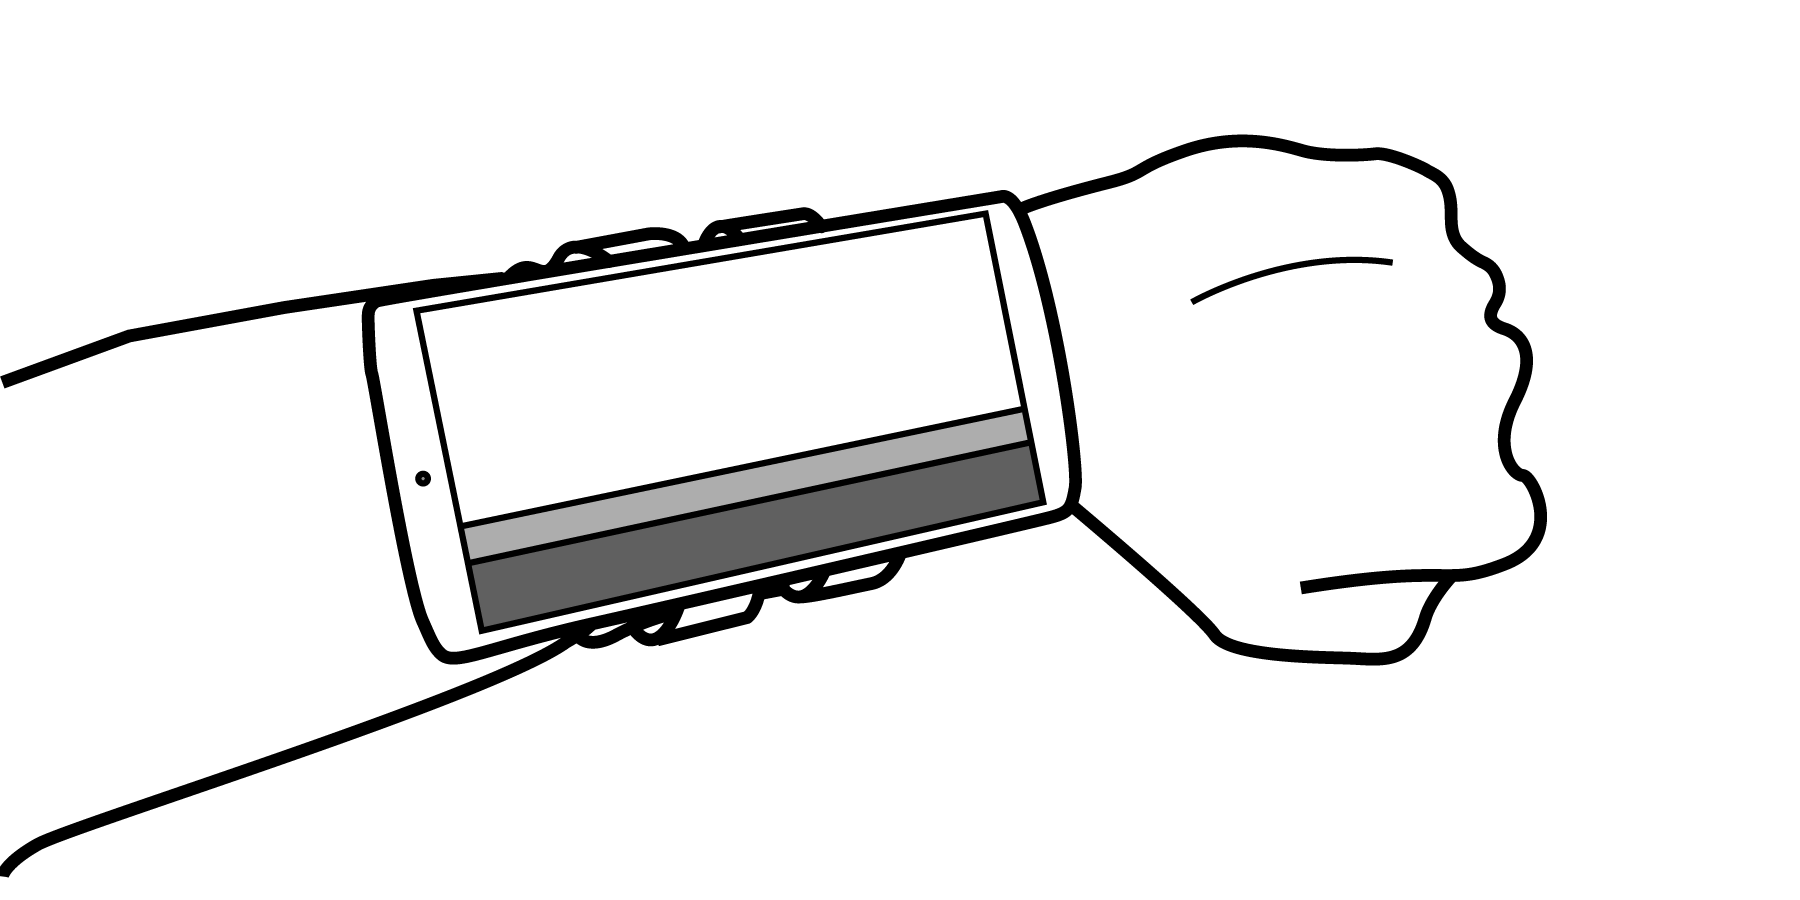
\includegraphics[width=85mm]{demo.png}
    \caption{smartphone bracelet for usage on wrists}
    \label{detection}
  \end{center}
\end{figure}

\end{document}
